\section{Rezerford tajribasi. Bor postulatlari}


\begin{enumerate}

\item ''Atom – bu musbat zaryad butun hajmi bo‘yicha teng taqsimlangan shar. Ushbu shar ichida elektronlar mavjud. Har bir elektron tebranish harakatlarini amalga oshirishi mumkin. Sharning musbat zaryadi modul bo‘yicha elektronlarning umumiy manfiy zaryadiga teng, shuning uchun atomning elektr zaryadi butunligicha nolga teng``. Qaysi olim atom tuzilishining bunday modelini taklif qilgan?
\begin{enumerate}[label=\Alph*)]
\item Albert Eynshteyn.
\item Ernest Rezerford.
\item Antuan Anri Bekkerel.
\item Jozef Jon Tomson.
\end{enumerate}

\item Rezerford qanday zarrachalarning yupqa moddalarda sochilishi orqali atomning yadro modelini tajriba orqali kashf etdi?
\begin{enumerate}[label=\Alph*)]
\item alfa zarralarning.
\item protonlarning.
\item gamma kvantlarning.
\item elektronlarning.
\end{enumerate}

\item Rezerford tajribasida $\alpha$-zarralar nima bilan ta’sirlashuv natijasida sochiladilar?
\begin{enumerate}[label=\Alph*)]
\item nishonning sirti bilan.
\item magnit maydon bilan.
\item yadro kuchlari maydoni bilan.
\item yadroning elektrostatik maydoni bilan.
\end{enumerate}

\item Atom radiusi atom yadrosi radiusidan taxminan necha marta katta?
\begin{enumerate}[label=\Alph*)]
\item $10^7$.
\item $10^5$.
\item $10^3$.
\item $10^2$.
\end{enumerate}

\item Vodorod atomidagi 4-statsionar orbitadagi elektronning tezligini toping (km/s).
\begin{enumerate}[label=\Alph*)]
\item 850.
\item 151.
\item 453.
\item 547.
\end{enumerate}

\item Vodorod atomidagi 3-statsionar orbitaning radiusini toping (\AA). 1-orbita radiusi 0,53 \AA.
\begin{enumerate}[label=\Alph*)]
\item 5,12.
\item 6,48.
\item 3,69.
\item 4,77.
\end{enumerate}

\item Vodorod atomidagi 5-statsionar orbitaning radiusini toping (\AA). 1-orbita radiusi 0,53 \AA.
\begin{enumerate}[label=\Alph*)]
\item 15,15.
\item 16,82.
\item 13,25.
\item 18,45.
\end{enumerate}

\item Rasmda atomning shartli statsionar elektron orbitalari tasvirlangan. Qaysi orbitada elektronlar eng katta energiyaga ega bo‘ladi? Qaysi orbitada elektronlar eng kichik energiyaga ega bo‘ladi?

\begin{center}
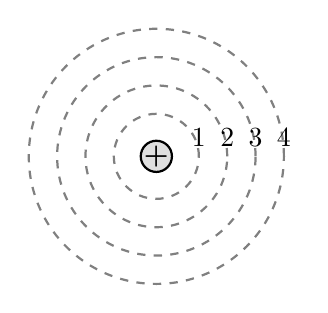
\begin{tikzpicture}[scale=0.9, >=stealth]
  % Musbat yadro (yadro markazi)
  \draw[fill=gray!25, thick] (0,0) circle (0.22) node {\textbf{+}};
  % Statsionar orbitalar (dashed lines)
  \draw[dashed, thick, gray] (0,0) circle (0.6);
  \draw[dashed, thick, gray] (0,0) circle (1.0);
  \draw[dashed, thick, gray] (0,0) circle (1.4);
  \draw[dashed, thick, gray] (0,0) circle (1.8);
  % Orbitalar raqamlari
  \node[above] at (0.6,0) {1};
  \node[above] at (1.0,0) {2};
  \node[above] at (1.4,0) {3};
  \node[above] at (1.8,0) {4};
\end{tikzpicture}
\end{center}

\begin{enumerate}[label=\Alph*)]
\item TJY.
\item 4-orbitada eng kichik, 1-orbitada eng katta.
\item 3-orbitada eng katta, 2-orbitada eng kichik.
\item 4-orbitada eng katta, 1-orbitada eng kichik.
\end{enumerate}

\item Vodorod atomidagi 3-statsionar orbitadagi elektronning energiyasini toping (eV). 1-orbitadagi energiyasi $-13,6$ eV ga teng.
\begin{enumerate}[label=\Alph*)]
\item -0,85.
\item -1,51.
\item -2,58.
\item -4,52.
\end{enumerate}

\item Vodorod atomidagi 6-statsionar orbitadagi elektronning energiyasini toping (eV). 1-orbitadagi energiyasi $-13,6$ eV ga teng.
\begin{enumerate}[label=\Alph*)]
\item -0,45.
\item -2,31.
\item -0,38.
\item -6,25.
\end{enumerate}

\item Atom $E_2$ energiyali holatdan $E_7$ energiyali holatga o‘tganida qanday energiyali fotonni yutadi?
\begin{enumerate}[label=\Alph*)]
\item $E_2$.
\item $E_7$.
\item $E_2 - E_7$.
\item $E_7 - E_2$.
\end{enumerate}

\item Atom $E_2$ energiyali holatdan $E_7$ energiyali holatga o‘tganida qanday chastotali fotonni yutadi?
\begin{enumerate}[label=\Alph*)]
\item $E_2/h$.
\item $E_7/h$.
\item $(E_2 - E_7)/h$.
\item $(E_7 - E_2)/h$.
\end{enumerate}

\item Atom $E_2$ energiyali holatdan $E_7$ energiyali holatga o‘tganida qanday to‘lqin uzunlikdagi fotonni yutadi?
\begin{enumerate}[label=\Alph*)]
\item $hc/(E_7 - E_2)$.
\item $hc/E_7$.
\item $hc/(E_2 - E_7)$.
\item $hc/E_2$.
\end{enumerate}

\item Vodorod atomidagi elektron 8-statsionar orbitadan 3-statsionar orbitaga o‘tdi. Quyidagi mulohazalardan qaysi biri to‘g‘ri?
\begin{itemize}
    \item[I.] Yutilgan foton energiyasi $E = E_8 - E_3$.
    \item[II.] Nurlangan foton energiyasi $E = E_8 - E_3$.
    \item[III.] Yutilgan foton energiyasi $E = E_8$.
    \item[IV.] Yutilgan foton energiyasi $E = E_3$.
\end{itemize}
\begin{enumerate}[label=\Alph*)]
\item I va II.
\item III va IV.
\item I va III.
\item faqat II.
\end{enumerate}

\item Vodorod atomidagi birinchi Bor orbitasi bo‘ylab harakatlanayotgan elektronning o‘rtacha kinetik energiyasi qanday (eV)?
\begin{enumerate}[label=\Alph*)]
\item 1,6.
\item 6,8.
\item 9,1.
\item 13,6.
\end{enumerate}

\item Vodorod atomidagi elektronning orbita bo‘ylab tezligi qanday (m/s)? $e=1,6\cdot 10^{-19}$ C; $m=9,1\cdot 10^{-31}$ kg; $r=10^{-8}$ cm; $k=9\cdot 10^9$ N$\cdot$m$^2$/kg$^2$.
\begin{enumerate}[label=\Alph*)]
\item $9\cdot 10^7$.
\item $9,1\cdot 10^6$.
\item $5,6\cdot 10^7$.
\item $1,6\cdot 10^6$.
\end{enumerate}

\item Chizmada keltirilgan atomning energetik sathlari orasidagi qaysi o‘tishda eng kichik chastotali foton yutiladi?

\begin{center}
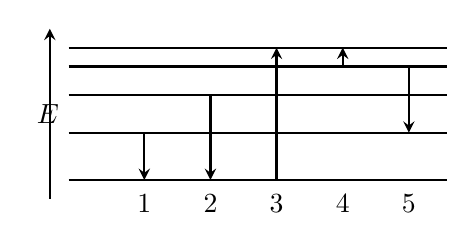
\begin{tikzpicture}[scale=1.2, >=stealth]
  % 5 ta energetik sath (energy levels)
  \draw[thick] (0,0) -- (4,0);
  \draw[thick] (0,0.5) -- (4,0.5);
  \draw[thick] (0,0.9) -- (4,0.9);
  \draw[thick] (0,1.2) -- (4,1.2);
  \draw[thick] (0,1.4) -- (4,1.4);
  
  \node[left] at (0, 0.7) {$E$};
  \draw[->, thick] (-0.2, -0.2) -- (-0.2, 1.6);

  % O'tishlar (transitions)
  % 1: level 2 -> level 1
  \draw[->, thick] (0.8, 0.5) -- (0.8, 0);
  
  % 2: level 3 -> level 1
  \draw[->, thick] (1.5, 0.9) -- (1.5, 0);
  
  % 3: level 1 -> level 5
  \draw[->, thick] (2.2, 0) -- (2.2, 1.4);
  
  % 4: level 4 -> level 5
  \draw[->, thick] (2.9, 1.2) -- (2.9, 1.4);
  
  % 5: level 4 -> level 2
  \draw[->, thick] (3.6, 1.2) -- (3.6, 0.5);

  % Raqamlar pastda
  \node[below] at (0.8, -0.05) {1};
  \node[below] at (1.5, -0.05) {2};
  \node[below] at (2.2, -0.05) {3};
  \node[below] at (2.9, -0.05) {4};
  \node[below] at (3.6, -0.05) {5};
\end{tikzpicture}
\end{center}

\begin{enumerate}[label=\Alph*)]
\item 1.
\item 2.
\item 3.
\item 4.
\end{enumerate}

\item Rasmda atom energetik sathlarining diagrammasi keltirilgan. Raqamli strelkalar bilan elektronning o‘tishlari berilgan. Elektron o‘tishlarining qaysi birida chastotasi eng kichik bo‘lgan foton nurlanadi?

\begin{center}
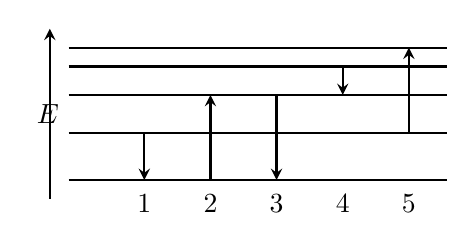
\begin{tikzpicture}[scale=1.2, >=stealth]
  % 5 ta energetik sath (energy levels)
  \draw[thick] (0,0) -- (4,0);
  \draw[thick] (0,0.5) -- (4,0.5);
  \draw[thick] (0,0.9) -- (4,0.9);
  \draw[thick] (0,1.2) -- (4,1.2);
  \draw[thick] (0,1.4) -- (4,1.4);
  
  \node[left] at (0, 0.7) {$E$};
  \draw[->, thick] (-0.2, -0.2) -- (-0.2, 1.6);

  % O'tishlar (transitions)
  % 1: level 2 -> level 1
  \draw[->, thick] (0.8, 0.5) -- (0.8, 0);
  
  % 2: level 1 -> level 3
  \draw[->, thick] (1.5, 0) -- (1.5, 0.9);
  
  % 3: level 3 -> level 1
  \draw[->, thick] (2.2, 0.9) -- (2.2, 0);
  
  % 4: level 4 -> level 3
  \draw[->, thick] (2.9, 1.2) -- (2.9, 0.9);
  
  % 5: level 2 -> level 5
  \draw[->, thick] (3.6, 0.5) -- (3.6, 1.4);

  % Raqamlar pastda
  \node[below] at (0.8, -0.05) {1};
  \node[below] at (1.5, -0.05) {2};
  \node[below] at (2.2, -0.05) {3};
  \node[below] at (2.9, -0.05) {4};
  \node[below] at (3.6, -0.05) {5};
\end{tikzpicture}
\end{center}

\begin{enumerate}[label=\Alph*)]
\item 5.
\item 4.
\item 3.
\item 2.
\end{enumerate}

\item Vodorod atomidagi elektron 3-statsionar orbitadan 2-statsionar orbitaga o‘tdi. Nurlangan foton chastotasini toping (Hz). Ridberg doimiysi $R=3,25\cdot 10^{15}$ Hz.
\begin{enumerate}[label=\Alph*)]
\item $\frac{R}{6}$.
\item $\frac{5R}{6}$.
\item $\frac{5R}{36}$.
\item $\frac{13R}{36}$.
\end{enumerate}

\item Vodorod atomidagi elektron 2-statsionar orbitadan 4-statsionar orbitaga o‘tdi. Yutilgan foton chastotasini toping (Hz). Ridberg doimiysi $R=3,25\cdot 10^{15}$ Hz.
\begin{enumerate}[label=\Alph*)]
\item $\frac{5R}{16}$.
\item $\frac{3R}{16}$.
\item $\frac{R}{16}$.
\item $\frac{R}{4}$.
\end{enumerate}

\item Vodorod atomidagi elektron birinchi holda 4-energetik sathdan 3-energetik sathga tushib, foton chiqardi. Ikkinchi holda 4-energetik sathdan 2-energetik sathga tushib, ikkinchi fotonni chiqardi. Bu ikki foton chastotalarining nisbati topilsin.
\begin{enumerate}[label=\Alph*)]
\item 7/27.
\item 7/108.
\item 14/27.
\item 7/54.
\end{enumerate}

\item Vodorod atomidagi elektron 4-energetik sathdan 2-energetik sathga tushdi va atom $\lambda_1$ to‘lqin uzunlikdagi, 3-energetik sathdan 1-energetik sathga tushsa $\lambda_2$ to‘lqin uzunlikdagi foton chiqardi. $\lambda_1 - \lambda_2$ ayirmaning qiymatini toping. Ridberg doimiysi $R=1,1\cdot 10^7\text{ m}^{-1}$.
\begin{enumerate}[label=\Alph*)]
\item $\frac{6}{65R}$.
\item $\frac{101}{24R}$.
\item $\frac{124}{47R}$.
\item $\frac{11}{114R}$.
\end{enumerate}

\item Vodorod atomlari 6-energetik sathgacha uyg‘otilgan. Bu gazning nurlanishida maksimal nechta spektral chiziqlar kuzatilishi mumkin?
\begin{enumerate}[label=\Alph*)]
\item 12.
\item 10.
\item 6.
\item 15.
\end{enumerate}

\item Vodorod atomi ultrabinafsha nurlar chiqarganda uning elektronlari qaysi statsionar orbitaga o‘tadi?
\begin{enumerate}[label=\Alph*)]
\item ikkinchi.
\item uchinchi.
\item birinchi.
\item to‘rtinchi.
\end{enumerate}

\item Vodorod atomidagi elektron uchinchi statsionar orbitaga o‘tsa, atom o‘zidan qanday to‘lqinlar chiqaradi?
\begin{enumerate}[label=\Alph*)]
\item infraqizil.
\item ko‘zga ko‘rinadigan.
\item rentgen.
\item ultrabinafsha.
\end{enumerate}

\end{enumerate}



\begin{table}[!ht]
\centering
\begin{tabular}{|c|c|c|c|c|c|c|c|c|c|c|}
\hline
1d & 2a & 3d & 4b & 5d & 6d & 7c & 8d & 9b & 10c & 11d \\ \hline
12d & 13a & 14d & 15d & 16d & 17d & 18b & 19c & 20b & 21a & 22b \\ \hline
23d & 24c & 25a & & & & & & & & \\ \hline
\end{tabular}
\end{table}